\documentclass[acmsmall,screen,review]{acmart}

\settopmatter{printacmref=false}
\setcopyright{none}
\renewcommand\footnotetextcopyrightpermission[1]{}
\acmConference[FSE Companion '27]{Draft for the FSE 2027 Industry Track}{July 2027}{Shenzhen, China}

\usepackage{xcolor}
\usepackage{booktabs}
\usepackage{tabularx}
\usepackage{draftwatermark}
\SetWatermarkText{IN PROGRESS}
\SetWatermarkScale{0.6}
\SetWatermarkLightness{0.92}

\newcommand{\todo}[1]{\textcolor{red}{\textbf{[TODO:} #1\textbf{]}}}
\newcommand{\prov}[1]{\textcolor{orange!85!black}{#1}}
\newcommand{\nmem}{\textsc{nmem}}

\begin{document}

\title{Recovering the Why Without Inventing It}
\subtitle{Grounded Decision Recovery from Repository History in Practice}

\author{Authors to be added}
\affiliation{\institution{Affiliation to be added}\country{Country}}

\begin{abstract}
Engineers who change unfamiliar code ask why it is the way it is. Part of the answer sits in pull requests, review
threads, and commit messages, scattered across years. Tools that turn a repository into readable pages answer such
questions fluently, including when the record holds no answer at all. We present \nmem{}, a system prepared for an internal pilot
that recovers decisions from a repository's history and shows each one with the record it came from. When nobody
wrote a reason down, \nmem{} says so and names the person to ask, instead of supplying a plausible reason. It checks
documentation by running the examples the documentation describes, and it weighs which decisions deserve a reader's
time. \nmem{} has built 11 public repositories in 10 languages, from 84 to 1,589 changes each.
\todo{One sentence each for RQ1 to RQ4 results, after human labels and the pilot.}
\end{abstract}

\keywords{software history, design rationale, mining software repositories, large language models, grounded generation}

\maketitle

\noindent\fbox{\parbox{\linewidth}{\small\textbf{Draft status, 17 Oct 2026.} Numbers in \prov{orange} are
provisional: they come from labels written by two models and are not yet replaced by human labels (Section~\ref{sec:design}).
Red notes mark missing work. References are not yet checked by a person and must not be cited as they stand.}}

\section{Introduction}

An engineer about to change a function needs to know whether its odd shape is an accident or a choice. The
reason, when one exists, is usually in the record: a pull request description, a review thread, an issue that
asked for the behavior, or a commit message. It is rarely where the engineer is looking. Reading it means knowing
which of thousands of changes touched the code, and which threads they named.

Generated repository documentation is now common. Tools such as DeepWiki~\cite{deepwiki2025} produce a browsable
wiki for any public repository. Research has started to generate design rationale with large language
models~\cite{llmdr2025}. Both answer the question \emph{why} in fluent prose. Neither is built to say that the
record holds no answer. For a reader deciding whether a behavior is safe to change, an invented reason is worse than
none. It is confident, it is plausible, and it cannot be checked.

\nmem{} takes the opposite stance. Every sentence it shows rests on a source in the repository record: a quoted
line of a pull request, a review comment, a commit, or a line of code at a named revision. The model never writes a
quote, a reference, a date, or a name. It returns handles, and code copies the text. A reason is shown only when a
quote states it and a second model call agrees that the quote states why. Otherwise the decision is shown with
``Nobody wrote down why'' and the person the record names as its author (Figure~\ref{fig:topic}).

This paper reports on \nmem{} in an industrial pilot. Its contributions are:
\begin{itemize}
  \item A pipeline that recovers decisions and their reasons from repository history under a grounding rule, with
        an explicit not-recorded outcome in place of a generated reason (Section~\ref{sec:system}).
  \item An evaluation on human-labelled decisions from real repositories, against showing every candidate and against
        a single-prompt baseline, with a held-out sample never used in tuning \todo{once labelled} (Section~\ref{sec:results}).
  \item A pilot with engineers that measures correctness, time, and confident wrong answers with and without
        \nmem{} \todo{once run}.
  \item Lessons from building and operating it on real repositories, and the code, labels, and scripts as an artifact.
\end{itemize}

\begin{figure}[t]
  \centering
  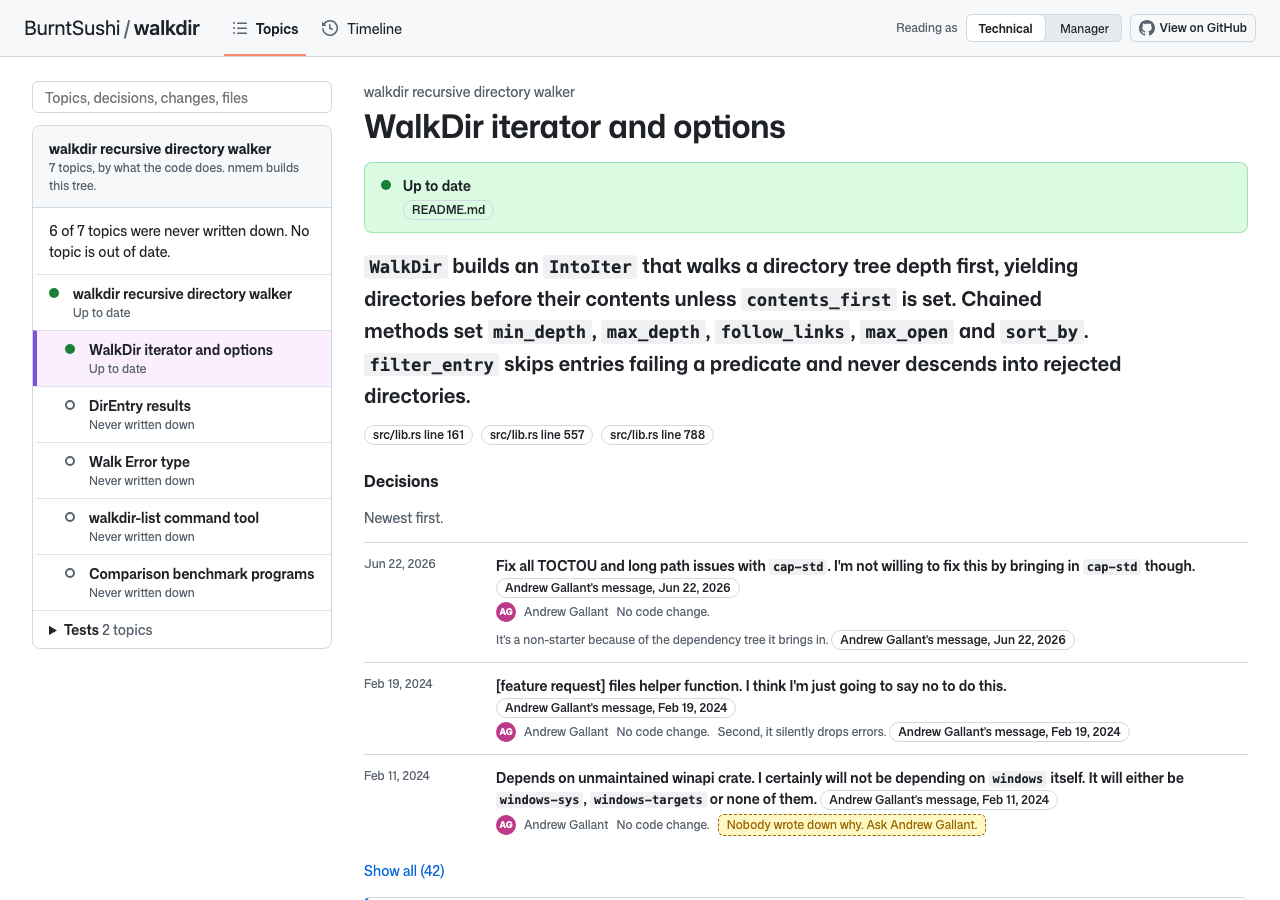
\includegraphics[width=\linewidth]{figs/topic.png}
  \caption{A topic page for BurntSushi/walkdir. Each decision links to the message it was quoted from. The third
  has no recorded reason, so \nmem{} says so and names who to ask.}
  \label{fig:topic}
  \Description{A web page listing a topic headline and three decisions with source chips, one marked "Nobody wrote down why. Ask Andrew Gallant."}
\end{figure}

\section{Context and related work}

\todo{A person reads each source before this section is written. Planned coverage:}
\begin{itemize}
  \item Rationale in software engineering: rationale in commit messages and developer discussion, and design
        decision mining from issue trackers. \todo{select and read the core papers.}
  \item LLM generation of design rationale~\cite{llmdr2025} and the datasets it builds on.
  \item Repository wiki generation~\cite{deepwiki2025}: retrieval-grounded pages and Q\&A, without a refusal to
        show unsourced reasons. \todo{confirm this characterisation from DeepWiki's own documentation.}
  \item Outdated documentation detection~\cite{docer2023emse,docer2023icsme}, which flags documentation that names
        code elements no longer in the repository. \nmem{} instead runs a program that tests the documented behavior.
\end{itemize}

\section{The \nmem{} system}
\label{sec:system}

\subsection{What it produces}
A build turns a git clone and the repository's GitHub record (pull requests, issues, discussions, reviews, tags, and
the authors of direct commits) into one snapshot. The snapshot holds:
\begin{itemize}
  \item \textbf{Changes}: each merged pull request or commit pushed straight to the default branch, classified as a
        decision carrier, a behavior change, a thing worth checking, routine, or quiet.
  \item \textbf{Decisions}: a choice the record states, the change that carried it, and its \emph{why}. The why is
        either \emph{recorded}, with a verified quote, or \emph{not recorded}, with the people to ask.
  \item \textbf{Topics}: a tree of what the code does, formed from the code at HEAD, each with a headline and a
        place to start reading.
  \item \textbf{Doc claims}: sentences in the documentation that the code decides, each marked up to date or out of
        date since a named change.
\end{itemize}
The web application reads the snapshot and renders a search-first front page, topic pages, a timeline, item
histories, and the quoted sources (Figure~\ref{fig:timeline}).

\subsection{Pipeline}
Table~\ref{tab:pipeline} lists the steps. Steps marked \emph{model} call a large language model through a cached
client. A rerun with the same inputs replays the cache and writes the same bytes.

\begin{table}[t]
\caption{The build pipeline.}
\label{tab:pipeline}
\small
\begin{tabularx}{\linewidth}{@{}lcX@{}}
\toprule
Step & Model & What it does \\
\midrule
ingest & no & Enumerate changes; cut records into sentences and lines with handles; flag denials, reverts, and bots. \\
prove & no & Prove routine files (docs, settings, version bumps, lockfiles, restyles, generated files) and add-then-undo groups. A change with only routine files is never sent to a model. \\
classify & yes & Per change, list sentences that could read as a choice, with a stance, plus behavior findings. \\
declined & yes & For threads no merged change carries that already read as a refusal, recover the refusal. \\
vet & yes & Drop a finding its record shows was handled, or that no user can reach. \\
link & yes & Join agreements in threads to the change that carried them. \\
why & yes & Keep a reason only with a verified quote and a second call that agrees it states why; else not recorded, with who to ask. \\
claims & yes & List doc sentences the code decides; where code can run, write a check program, run it at HEAD and at each change since, and date the break. \\
topics & yes & Form the topic tree from HEAD; write each page; place decisions and findings on topics. \\
weigh & yes & Mark each decision key, minor, or not a decision; drop the last. \\
assemble & no & Copy verified quotes into the snapshot, validate it, write. \\
\bottomrule
\end{tabularx}
\end{table}

\subsection{Grounding rules}
Three rules hold across every step. First, the model never writes a quote, reference, login, change identifier, line
number, or date; it returns handles to sentences and lines, and code copies the text, so a shown quote is always a
substring of the record. Second, every object with a not-recorded reason is scanned once more for any sentence that
states a reason as fact; a flagged sentence is dropped, and a flagged decision is dropped whole. Third, each model
step has one honest fallback, and a build that loses its model provider fails instead of writing a partial snapshot.

\subsection{Operation}
A worker process builds repositories on request, one at a time, and survives restarts. Within minutes it publishes a
first snapshot built without the model, so the pages open before the full build ends. \todo{Deployment and access
for the pilot, once decided.}

\begin{figure}[t]
  \centering
  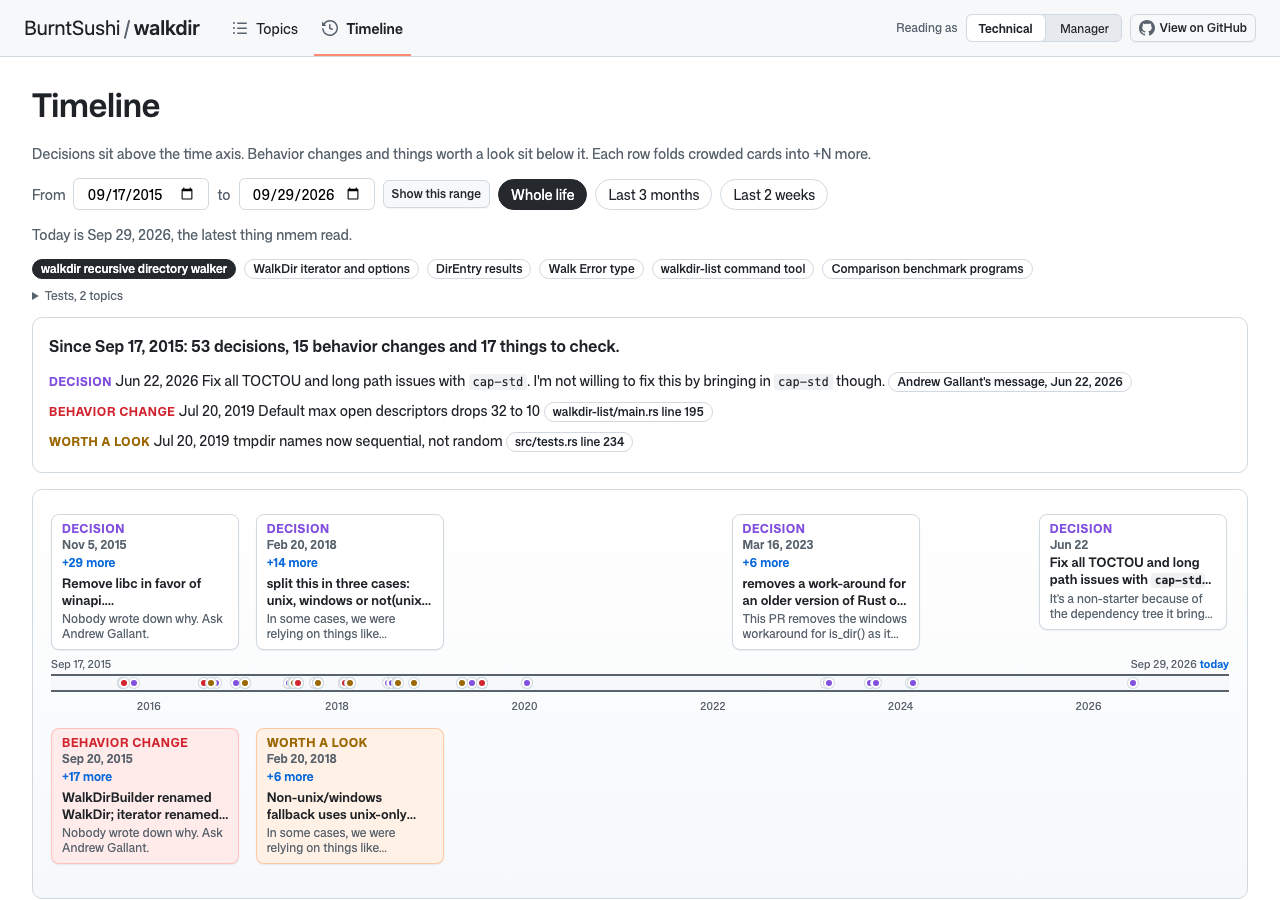
\includegraphics[width=\linewidth]{figs/timeline.png}
  \caption{The timeline for BurntSushi/walkdir. Decisions sit above the axis, behavior changes and things worth a
  look below it.}
  \label{fig:timeline}
  \Description{A timeline with decision cards above a date axis and behavior change cards below it.}
\end{figure}

\section{Evaluation design}
\label{sec:design}

\subsection{Research questions}
\begin{description}
  \item[RQ1] How precisely and completely does \nmem{} surface the decisions worth a reader's attention?
  \item[RQ2] How often is a shown reason unsupported by its source, and how often is ``not recorded'' correct?
  \item[RQ3] How often is an out-of-date doc flag right?
  \item[RQ4] Do engineers answer history questions more accurately or faster with \nmem{}, and how often are they
             confident and wrong?
  \item[RQ5] What does a build cost in model calls and time?
\end{description}

\subsection{Data}
\textbf{Decision sample.} We sampled 35 decisions at random from each of six repositories (210 in all, seed
20261015): mozilla-ai/agent-factory, apple/swift-argument-parser, and square/javapoet for development, and
expressjs/body-parser, rack/rack-attack, and mat/besticon held out. A rubric asks whether each entry deserves a reader's
attention, as a key or minor choice, or is not a decision.
\prov{The current labels were written by two models, with disagreements on 26 of 210 settled by a third model run.}
\todo{Two human labellers relabel all 210 blind to the model labels; report Cohen's kappa. Draw and label a fresh
held-out sample of 140 from four repositories never used in tuning.}

\textbf{Synthetic fixtures.} Generated repositories with planted decisions, gaps, and doc claims give a controlled
check of the grounding rules, including a count of invented reasons. \todo{Describe the generator and the scoring
rows from the harness design.}

\textbf{Baselines.} Showing every candidate decision (the pipeline without the weigh step), and \todo{a single prompt per
change that lists decisions and reasons, on the same model, with no grounding check}.

\textbf{Pilot.} 8 to 12 engineers, within subjects and counterbalanced: four timed tasks with \nmem{} and four with
GitHub alone, one of each kind (a recorded why, an unrecorded why, doc currency, and finding a change), then two weeks
of free use and an interview. \todo{Recruitment, consent, and results.}

\section{Results}
\label{sec:results}

\subsection{RQ1: decision recovery}
Table~\ref{tab:rq1} gives the current scores. Precision is the share of kept sampled decisions that are worth showing.
Recall is the share of worth-showing sampled decisions that are kept. The weigh step was tuned on the development
repositories only, and the held-out repositories were scored once.

\begin{table}[t]
\caption{Decision recovery against the \prov{model-labelled} sample. Measured 17 Oct 2026 with
\texttt{harness/decisions-real.mjs}.}
\label{tab:rq1}
\small
\begin{tabular}{@{}lrrrrr@{}}
\toprule
Split & Shown & Sampled & Kept & Precision & Recall \\
\midrule
Development (3 repos) & 630 & 105 & 39 & \prov{76.9\%} & \prov{90.9\%} \\
Held out (3 repos) & 235 & 105 & 21 & \prov{85.7\%} & \prov{81.8\%} \\
\midrule
Show everything, held out & -- & 105 & 105 & \prov{21.0\%} & 100\% \\
\bottomrule
\end{tabular}
\end{table}

\todo{Replace with human labels, add the fresh held-out sample and the single-prompt baseline, and report
confidence intervals.}

\subsection{RQ2 and RQ3: faithfulness and doc currency}
\todo{Human labels on 100 shown reasons and 100 not-recorded entries, mixed blind with baseline answers. Precision of
out-of-date flags on a sample.}

\subsection{RQ4: the pilot}
\todo{Correctness, time, confident-and-wrong counts, and interview themes.}

\subsection{RQ5: cost}
Table~\ref{tab:cost} lists the repositories built for the pilot. Model calls ran 2.5 to 10 per change. A cold build of
BurntSushi/walkdir took 12.9 minutes with 4 model calls in flight and 5.4 minutes with 16, with no rate limiting from
the provider. JamesNK/Newtonsoft.Json, the largest, took 76 minutes cold. Each timing is a single run.
\todo{Add tokens per change from the build logs, and repeat the timings three times.}

\begin{table}[t]
\caption{Repositories built for the pilot. Decisions are those shown after the weigh step.}
\label{tab:cost}
\small
\begin{tabular}{@{}llrrr@{}}
\toprule
Repository & Language & Changes & Model calls & Decisions \\
\midrule
sindresorhus/p-limit & TypeScript & 84 & 369 & 18 \\
BurntSushi/walkdir & Rust & 185 & 928 & 53 \\
mozilla-ai/agent-factory & Python & 191 & 2,060 & 236 \\
phpdotenv \todo{owner} & PHP & 339 & 1,568 & 69 \\
rack/rack-attack & Ruby & 479 & 2,087 & 121 \\
square/javapoet & Java & 522 & 2,335 & 131 \\
apple/swift-argument-parser & Swift & 538 & 2,780 & 263 \\
mat/besticon & Go & 546 & 2,214 & 56 \\
expressjs/body-parser & JavaScript & 737 & 2,276 & 58 \\
pallets/click & Python & 1,384 & 6,962 & 528 \\
JamesNK/Newtonsoft.Json & C\# & 1,589 & 7,826 & 262 \\
\bottomrule
\end{tabular}
\end{table}

\section{Lessons learned}
\todo{Keep only lessons the data supports. Candidates:}
\begin{itemize}
  \item A filter that raised scores on the synthetic fixtures removed true behavior changes on real repositories
        (14 of 14 findings it dropped were real), and was removed. Fixtures alone mislead tuning.
  \item Distinguishing ``read and found nothing worth showing'' from ``could not classify'' changed what users saw:
        on one repository, 165 of 339 changes had shown as unclassified.
  \item Opening pages from a model-free snapshot within minutes changed how people approached a cold repository.
        \todo{support with pilot data.}
  \item Naming who to ask fails for bots and email-only commits, which carry no account to name.
\end{itemize}

\section{Threats to validity}
\todo{Sample sizes; one company; public repositories only; labels replaced late in the project; model and provider
dependence; cost.}

\section{Conclusion}
\todo{After results.}

\section*{Use of AI tools}
\todo{State how AI tools were used in writing this paper and in building the system, per ACM's authorship policy.
Large language models are a component of \nmem{} (Section~\ref{sec:system}). Drafts of this paper were written with
an AI coding assistant and are being checked and rewritten by the authors.}

\section*{Artifact}
\todo{Link to the code, the labelled samples, and the scripts that produce every table.}

\bibliographystyle{ACM-Reference-Format}
\bibliography{refs}

\end{document}
